
\chapter{Background}\label{chap:background}
This chapter introduces the main concepts and technologies that are the base of this dissertation.\\
We will start by introducing the Phase Change Memory (PCM), a non-volatile memory (NVM) capable of storing data by changing the state of the material, 
and why it is suitable for this kind of application.
Then we will introduce the concept of Analog In-Memory Computing (AIMC) and how it can be used to speed up matrix-vector multiplication.\\
Finally we will introduce the PULP platform and the GVSoC simulator as the tools and frameworks for the module implementation.
\newpage
\section{Phase Change Memory (PCM)}\label{sec:pcm}

Phase Change Memory (PCM) \picref{fig:PCM-Cell-Schematics} is a type of NVM that uses the unique behaviour of some chalcogenide 
  compound materials to switch between amorphous and crystalline states, 
  these two phases offer differential electrical impedance that manifests as variable resistance \cite{gallo_overview_2020,he_-memory_2023}.
By applying a current to the material we can measure the output voltage and, by using Ohm's law, 
we can determine the resistance of the material and therefore the value of the cell.
The state change is achieved by applying different heat levels to the material using electrical pulses \picref{fig:PCM-Set-and-Reset}; 
these pulses differ in both intensity and duration depending on the desired state.
For this exact reason we can notice a difference in write and read speed, 
with writes being slower and of variable durations but allowing reading speed comparable to DRAM read speed, or of around 50 ns \cite{srinivasan_study_2013}.\\

By reviewing the literature we can find papers starting to describe this innovation as early as 1960s however in the following decade the interest 
  declined until the 2000s as drift related issues emerged. In the early 2000 the technology started to be developed for commercial use, one widely recognized implementation is the Intel Optane, a PCM based technologies called 3D XPoint \cite{gallo_overview_2020,he_-memory_2023}.
Initially conceived as a binary memory technology, PCM has evolved to support multi-level cell architectures by using multiple levels of resistance to rappresent the stored data \cite{antolini_readout_2024}.
This property makes PCM particularly suitable for MVM and MM operations, as the weights of the matrices can be stored as resistance values directly within the memory cells.

\begin{figure}[H]
  \centering
  \subfloat[PCM Cell Schematics. Adapted from \cite{mannocci_-memory_2023}]{
    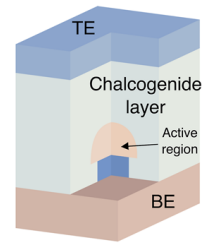
\includegraphics[height=5cm,keepaspectratio]{Figures/Cell Schematics.png}
    \label{fig:PCM-Cell-Schematics}
  }
  \hspace{1cm} 
  \subfloat[PCM Set and Reset pulses. Adapted from \cite{wuttig_phase-change_2007}]{
    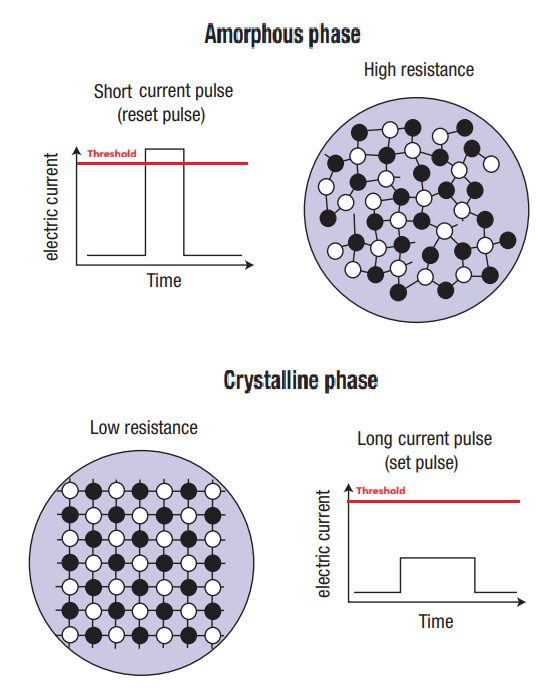
\includegraphics[height=5cm,keepaspectratio]{Figures/Set and Reset.png}
    \label{fig:PCM-Set-and-Reset}
  }
  \caption{PCM Cell Schematic and Set/Reset Pulses.}
  \label{fig:PCM-cell-and-pulses}
\end{figure}

\section{Analog In-Memory Computing (AIMC)}\label{sec:aimc}
With Analog In-Memory Computing (AIMC) we refer to a computing paradigm that aims to perform computations directly within the memory array, 
  thus reducing the need for data movement between memory and processing units.
This approach is particularly beneficial for operations that involve large amounts of data, such as matrix-vector multiplications (MVMs) 
and matrix-matrix multiplications (MMs), which are common in machine learning, AI and scientific computing applications.\\
AIMC leverages the physical properties of memory devices, such as resistive switching in PCM, to perform computations in an analog manner.
This allows for parallel processing of multiple operations by design, leading to significant speedups compared to traditional digital computing approaches.
Moreover, analog capabilities scales better than digital operations leading to improved energy efficiency as the data grows.

\section{Applying AIMC to PCM}\label{sec:aimc_pcm}
The PCM technology is particularly interesting for AIMC because it allows parallel execution of multiple operations.
In fact, the internal structure of PCM crossbar-array \picref{fig:PCM-module-and-structure} allows to perform matrix-vector multiplications (MVMs) in a single step:
by applying the input vector as current $X_i$ to the rows of the PCM array and reading the output current from the columns, thanks to Kirchhoff's law,
we retrieve the result $Y_i = \sum_{k=0}^{n} X_i \cdot R_{ik}$ in a single operation \cite{he_-memory_2023}.\\
Moreover, the AIMC capability of a PCM crossbar make good use of the reading operation, which is significantly faster than the writing operation optimising the overall performance for such computations.
To apply this concept to a real PCM module we need to consider some additional aspects such as the presence of Digital-to-Analog Converters (DACs) 
  to convert the digital input vector to analog signals for the rows and Analog-to-Digital Converters (ADCs) to convert the analog output currents from the columns back to digital values.

\subsection{PCM Module Architecture}\label{sec:PCM_Module_arch}
After considering the PCM cell architecture and its internal schematics we can now analyse the structure of a PCM module that can be used for AIMC.
The PCM module architecture is shown in figure \picref{fig:PCM-Module-Architecture}.\\
The module is characterised by a matrix $R\;\times\;C$ of tiles. Each tile is a 3D array itself with surface $X \;\times\; Y$ and depth $K$, with $K$ being the 
number of layers of PCM cells stacked on top of each other. Each cell is able to holds $n$-bits as variable resistance. 
The core concept of the entire module is to hold up to $L$ layers, as $L = C \cdot K$, stored as $X\;\times\;J\;$ matrices, with being $J=Y\cdot R$. 
During a computations is possible to select layers and matrices portions, 
called sectors, to use by providing the module with specific commands on the data bus.
The tiles are interfaced with a set of DACs connected to the rows and ADCs connected to the columns, enabling bidirectional conversion of input vectors from digital to analog and output vectors from analog to digital, respectively.
This is the basic architecture of the PCM module that we will use for our implementation.

\begin{figure}[!tbh]
\begin{minipage}{.5\textwidth}
    \subfloat[PCM Memory Architecture]{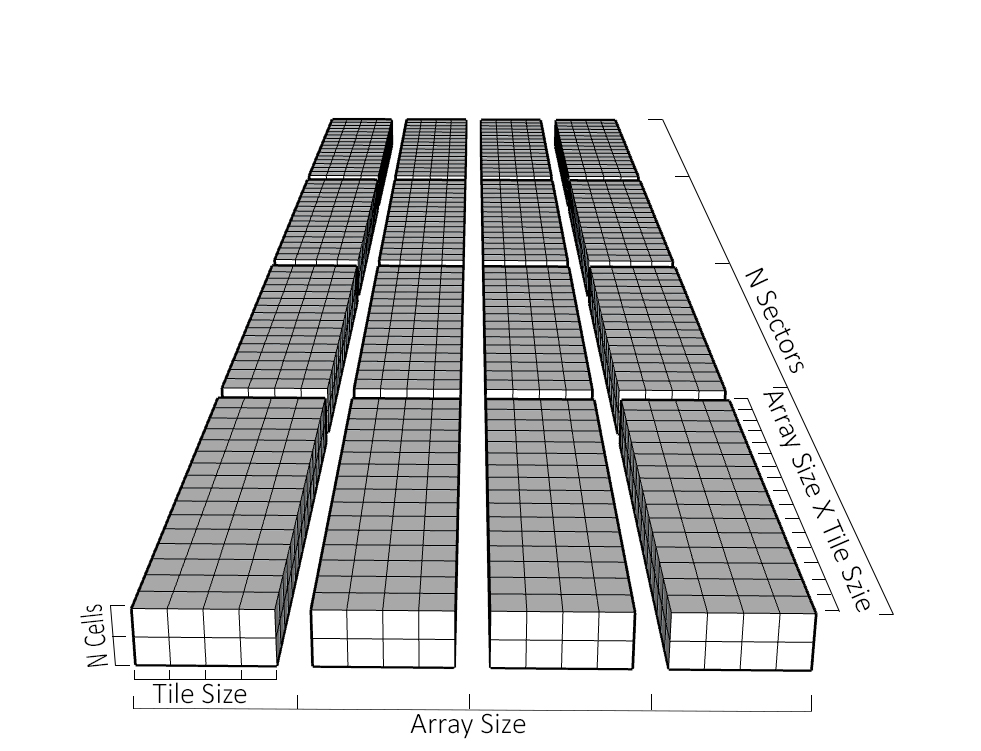
\includegraphics[width=\textwidth]{Figures/Memory Architecture.jpg}
    \label{fig:PCM-Module-Architecture}}
\end{minipage}
\hfill    
\begin{minipage}{.5\textwidth}
    \subfloat[PCM Internal Schematics. Adapted from \cite{he_-memory_2023}]{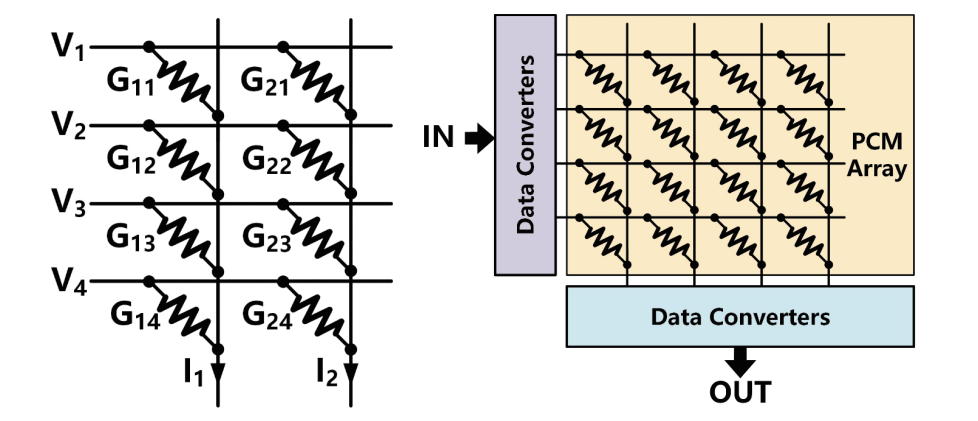
\includegraphics[width=\textwidth]{Figures/PCM Schematics.png}\label{fig:PCM-Internal-Schematics}}
\end{minipage}
    \caption{\\ PCM Module Architecture and Structure. }
    \label{fig:PCM-module-and-structure}
\end{figure}


\section{PULP Platform}\label{sec:pulp}
Parallel Ultra Low Power (PULP) is an open-source computing platform developed by the PULP team at the University of Bologna and the ETH Zurich.

\subsection{PULP Overview}\label{sec:pulp_ov}%Too much PULP?
The platform's objective is to provide high performance and energy efficient computing solutions based on the RISC-V architecture.
Within the platform we can find a variety of processing units, including RISC-V cores and specialized accelerators.
The framework is highly configurable, allowing designers to tailor the architecture to specific application requirements.
PULP is particularly well-suited for edge computing applications, where power consumption and performance are critical factors.
\subsection{GVSoC Simulator}\label{sec:gvsoc}
The PULP ecosystem is supported by a complete software stack, including the SoC simulator (GVSoC) \cite{bruschi_gvsoc_2021},
 which provides an event-driven simulation environment for PULP-based systems.
This simulator allows developers to model and simulate the behavior of systems on chip, enabling them to evaluate performance,
 power consumption, and other metrics before deploying on actual hardware.
GVSoC supports a wide range of features, including multi-core processing, SoC clusters, memory hierarchies, and peripheral devices.
Within GVSoC, developers can create virtual prototypes of custom hardware modules, such as the PCM module described in this dissertation,
and integrate them into the PULP platform for simulation and testing.
We’ll cover this in the upcoming chapters.
